\documentclass[11pt]{article}

% ---------- layout & fonts ----------
\usepackage[margin=1in,headheight=14pt]{geometry}
\usepackage[T1]{fontenc}
\usepackage{libertinus}
\usepackage[scale=0.95]{sourcesanspro}
\renewcommand{\familydefault}{\rmdefault}
\usepackage{microtype}
\usepackage{amsmath,amssymb}
\usepackage{graphicx}
\usepackage{booktabs}
\usepackage{tabularx}
\usepackage[table]{xcolor}
\usepackage[font=small,labelfont={bf,color=bbnavy},labelsep=period]{caption}
\usepackage{enumitem}
\usepackage{titlesec}
\usepackage{fancyhdr}
\usepackage[most]{tcolorbox}
\usepackage{fontawesome5}
\usepackage{tikz}
\usetikzlibrary{arrows.meta,positioning,shadows}
\usepackage[colorlinks=true,linkcolor=bbteal,citecolor=bbteal,urlcolor=bbteal]{hyperref}

% ---------- colours (match the BreathBreak slides and app) ----------
\definecolor{bbnavy}{HTML}{12294A}
\definecolor{bbteal}{HTML}{0E8A8F}
\definecolor{bbcoral}{HTML}{F2685B}
\definecolor{bbamber}{HTML}{F5A623}
\definecolor{bblight}{HTML}{E8F4F4}
\definecolor{bbgrey}{HTML}{5B6573}

% ---------- headings: chapters of the story ----------
\titleformat{\section}{\sffamily\Large\bfseries\color{bbnavy}}{\color{bbteal}Chapter \thesection}{0.6em}{\color{bbgrey}·\ \color{bbnavy}}
\titleformat{name=\section,numberless}{\sffamily\Large\bfseries\color{bbnavy}}{}{0pt}{}
\titleformat{\subsection}{\sffamily\large\bfseries\color{bbnavy}}{}{0pt}{}
\titleformat{\paragraph}[runin]{\sffamily\bfseries\color{bbteal}}{}{0pt}{}
\titlespacing*{\section}{0pt}{20pt}{8pt}
\titlespacing*{\subsection}{0pt}{12pt}{5pt}

% ---------- header / footer ----------
\pagestyle{fancy}
\fancyhf{}
\fancyhead[L]{\sffamily\small\color{bbteal}\textbf{BreathBreak}\color{bbgrey}\ \ ·\ \ the story}
\fancyhead[R]{\sffamily\small\color{bbgrey}UTD HackEdge 2026 \,·\, Track 1}
\fancyfoot[C]{\sffamily\small\color{bbgrey}\thepage}
\renewcommand{\headrulewidth}{0.4pt}
\renewcommand{\headrule}{\hbox to\headwidth{\color{bbteal}\leaders\hrule height \headrulewidth\hfill}}

\renewcommand{\arraystretch}{1.15}
\newcommand{\rowband}{\rowcolors{2}{bblight}{white}}

% ---------- boxes ----------
\newtcolorbox{keybox}[1]{enhanced,colback=bblight,colframe=bbteal,boxrule=0.8pt,arc=3pt,
  fonttitle=\sffamily\bfseries,coltitle=white,colbacktitle=bbteal,title={#1},left=8pt,right=8pt,top=6pt,bottom=6pt}
\newtcolorbox{twistbox}[1]{enhanced,colback=bbcoral!6,colframe=bbcoral,boxrule=0.8pt,arc=3pt,
  fonttitle=\sffamily\bfseries,coltitle=white,colbacktitle=bbcoral,title={#1},left=8pt,right=8pt,top=6pt,bottom=6pt}
\newtcolorbox{lessonbox}{enhanced,colback=bbamber!8,colframe=bbamber,boxrule=0pt,leftrule=3pt,arc=0pt,
  left=8pt,right=8pt,top=5pt,bottom=5pt,fontupper=\sffamily\small}
\newcommand{\lesson}[1]{\begin{lessonbox}\textbf{\color{bbnavy}What we learned:}\ #1\end{lessonbox}}

\graphicspath{{outputs/comparison/}{./}}
\setlist{itemsep=2pt,topsep=4pt}

\begin{document}

% =====================================================================
% title page
\thispagestyle{empty}
\begin{tikzpicture}[remember picture,overlay]
  \shade[left color=bbnavy,right color=bbteal] (current page.north west) rectangle ([yshift=-7.6cm]current page.north east);
  \fill[bbamber] ([yshift=-7.6cm]current page.north west) rectangle ([xshift=6cm,yshift=-7.8cm]current page.north west);
  \fill[bbcoral] ([xshift=6cm,yshift=-7.6cm]current page.north west) rectangle ([xshift=9cm,yshift=-7.8cm]current page.north west);
  % ECG trace across the banner
  \draw[color=green!70!teal, line width=1.4pt, line join=round]
    ([yshift=-6.4cm]current page.north west)
    \foreach \i in {0,...,6} { -- ++(1.6,0) -- ++(0.15,0.25) -- ++(0.15,-0.25) -- ++(0.2,0) -- ++(0.08,-0.2)
      -- ++(0.1,1.3) -- ++(0.12,-1.6) -- ++(0.1,0.5) -- ++(0.5,0) -- ++(0.25,0.35) -- ++(0.25,-0.35) };
  \node[anchor=north west,text width=15.5cm,align=left] at ([xshift=2.5cm,yshift=-1.3cm]current page.north west) {%
    {\sffamily\bfseries\color{bbamber} UTD HACKEDGE 2026 \,·\, EDGE AI TRACK}\\[10pt]
    {\sffamily\bfseries\fontsize{38}{40}\selectfont\color{white} BreathBreak}\\[10pt]
    {\sffamily\Large\color{white} The story of a small pause:\\ detecting fatigue from your own heartbeat, at the edge}};
\end{tikzpicture}
\vspace*{6.1cm}

{\sffamily
\begin{tabularx}{\textwidth}{@{}X r@{}}
\textbf{\color{bbnavy}Nhat Truong \,·\, Dung Anh Nguyen \,·\, Anthony Tran} & \color{bbgrey}November 2026\\[2pt]
\color{bbgrey}\faGithub\ \href{https://github.com/nhattruong0205/HackEdge}{github.com/nhattruong0205/HackEdge} & \\
\end{tabularx}}

\vspace{14pt}
\begin{tcolorbox}[enhanced,colback=white,colframe=bbteal,boxrule=0.8pt,arc=3pt,left=10pt,right=10pt,
  title={\sffamily\bfseries The story in one paragraph},colbacktitle=bbteal,coltitle=white]
We set out to build a wearable that notices when a worker on a long shift is getting dangerously tired and
suggests a two-minute breathing break. Our first surprise was that raw ECG features mostly tell you
\emph{who} is wearing the sensor, not how tired they are. Our second was that the \emph{change} from a
person's own healthy rest is large and consistent: heart rate up by about half, beat-to-beat variability
down by three quarters. A four-parameter model built on that idea beat transfer learning from public
datasets and runs entirely on a TI SK-AM62B. Then the data surprised us a third time: recordings labelled
``normal'' were taken while one of us was sick, and a sick body already looks fatigued. That taught us what
BreathBreak can and cannot see, why a healthy baseline matters, and why we chose to tolerate a missed alert
rather than a false alarm.
\end{tcolorbox}

\begin{keybox}{\faChartLine\ \ The story in numbers}
\begin{tabularx}{\linewidth}{@{}>{\centering\arraybackslash}X >{\centering\arraybackslash}X >{\centering\arraybackslash}X >{\centering\arraybackslash}X@{}}
{\sffamily\bfseries\huge\color{bbcoral}+58\%} & {\sffamily\bfseries\huge\color{bbnavy}$-$78\%} & {\sffamily\bfseries\huge\color{bbteal}11/11} & {\sffamily\bfseries\huge\color{bbteal}0} \\
\small heart-rate rise, rest $\rightarrow$ fatigue (subject A) & \small RMSSD drop, rest $\rightarrow$ fatigue (subject A) &
\small leave-one-out, healthy rest vs.\ fatigue & \small false alarms on rested recordings \\
\end{tabularx}
\end{keybox}

\newpage
% =====================================================================
\section{Hour eleven}

Picture a nurse eleven hours into a twelve-hour shift, a truck driver on the last leg of a night run, a
factory worker at the end of a double. None of them feels a switch flip from ``alert'' to ``dangerous''.
Fatigue builds slowly, and by the time it is obvious, the mistake has often already happened. Prolonged
wakefulness impairs performance about as much as alcohol does \cite{williamson2000}, yet at most
workplaces fatigue is managed with fixed schedules and a ``tell us if you're tired'' policy.

Our idea was simple: \textbf{a small pause is better than a big accident}. If a wearable could notice the body
drifting into fatigue, it could suggest a two-minute breathing break at the right moment, and, in aggregate,
show managers which shifts wear people down. We called it \emph{BreathBreak}.

\begin{figure}[h]
\centering
\fbox{\includegraphics[page=3,width=0.8\linewidth,trim=0 40 0 95,clip]{breathbreak-slides.pdf}}
\caption{The BreathBreak concept: real-time break alerts for the worker, workload reports for HR.}
\end{figure}

Two constraints shaped everything that followed. Heart data are personal, and worksites often have poor
connectivity, so the decision had to be made \emph{on the device}, at the edge, not in the cloud. And a
system that interrupts people at work has to earn their trust: \textbf{every false alarm teaches a worker
to ignore the next one}.

% =====================================================================
\section{Listening to the heart}

The heart is a good witness. When we are rested and calm, the parasympathetic (``rest and digest'') branch
of the nervous system keeps the heart rate low and lets it wander slightly from beat to beat. Under strain,
the sympathetic branch takes over: the heart beats faster and more like a metronome
\cite{taskforce1996,shaffer2017}. Three numbers capture this:

\begin{itemize}
  \item \textbf{Heart rate (HR)}, in beats per minute;
  \item \textbf{SDNN}, the overall spread of the intervals between beats;
  \item \textbf{RMSSD}, how much consecutive beats differ: the fastest-reacting marker of the calming branch.
\end{itemize}

We recorded ECG with a \textbf{TI AFE4950} front end at 500~Hz and built a pipeline to turn raw voltage into
those numbers: zero-phase filtering (0.5~Hz high-pass, 60~Hz notch, 40~Hz low-pass), masking of motion
spikes, Pan--Tompkins R-peak detection \cite{pantompkins1985}, cleaning of implausible beat intervals, and
trimming of the unstable start and end of each recording.

\begin{figure}[h]
\centering
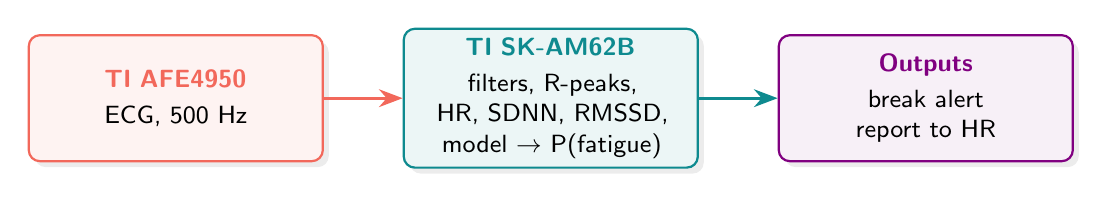
\begin{tikzpicture}[node distance=1.0cm, every node/.style={font=\sffamily\small},
  box/.style={rounded corners=4pt, align=center, minimum height=1.6cm, text width=3.5cm, thick, drop shadow={opacity=.15}}]
  \node[box, draw=bbcoral, fill=bbcoral!8] (afe) {\textbf{\color{bbcoral}TI AFE4950}\\[2pt]ECG, 500 Hz};
  \node[box, draw=bbteal, fill=bbteal!8, right=of afe] (edge) {\textbf{\color{bbteal}TI SK-AM62B}\\[2pt]filters, R-peaks,\\HR, SDNN, RMSSD,\\model $\rightarrow$ P(fatigue)};
  \node[box, draw=violet, fill=violet!6, right=of edge] (out) {\textbf{\color{violet}Outputs}\\[2pt]break alert\\report to HR};
  \draw[-{Stealth[length=3mm]}, very thick, bbcoral] (afe) -- (edge);
  \draw[-{Stealth[length=3mm]}, very thick, bbteal] (edge) -- (out);
\end{tikzpicture}
\caption{From heartbeat to break alert. Everything after acquisition runs on the edge board.}
\end{figure}

% =====================================================================
\section{The first surprise: the data knew who we were}

Our first instinct was the standard one: compute a set of features from each recording and train a
classifier to say \emph{normal} or \emph{fatigue}. It didn't work, and the reason was instructive.

The two people in our data, whom we call \textbf{A} and \textbf{B}, have very different hearts. A's R-peak
is about 32~mV tall, B's about 46~mV; the shape of the T-wave differs too, and even moving the electrodes a
few centimetres between sessions changes the waveform. Worse, those shape features moved in
\emph{opposite} directions in the two people between rest and fatigue. A classifier on absolute values
would mostly learn \emph{who is wearing the sensor}.

\lesson{absolute ECG features identify the person. To detect a \emph{state}, we have to compare each person
with themselves.}

% =====================================================================
\section{The idea: compare you with you}

So we looked at the \emph{change} from each person's own rested state instead. Here the picture was
strikingly clear (Figure~\ref{fig:shift}): in both people, fatigue moved every heart-rate and HRV measure in
the same direction, with very large effects ($p<10^{-4}$).

\begin{table}[h]
\centering
\caption{Rest vs.\ fatigue within each person (20-s windows; values from our technical report, where
subject B is called C).}
\label{tab:shift}
\rowband\begin{tabular}{lrrrrr}
\toprule
 & \multicolumn{2}{c}{Subject A} & \multicolumn{2}{c}{Subject B} & \\
\cmidrule(lr){2-3}\cmidrule(lr){4-5}
Measure & Rest & Fatigue & Rest & Fatigue & Change \\
\midrule
Heart rate (bpm) & 67.1 & 105.6 & 77.5 & 106.0 & $+37$ to $+58\%$ \\
SDNN (ms)        & 38.3 & 16.7  & 44.5 & 14.7  & $-56$ to $-67\%$ \\
RMSSD (ms)       & 36.1 & 8.1   & 32.1 & 10.4  & $-68$ to $-78\%$ \\
\bottomrule
\end{tabular}
\end{table}

\begin{figure}[h]
\centering
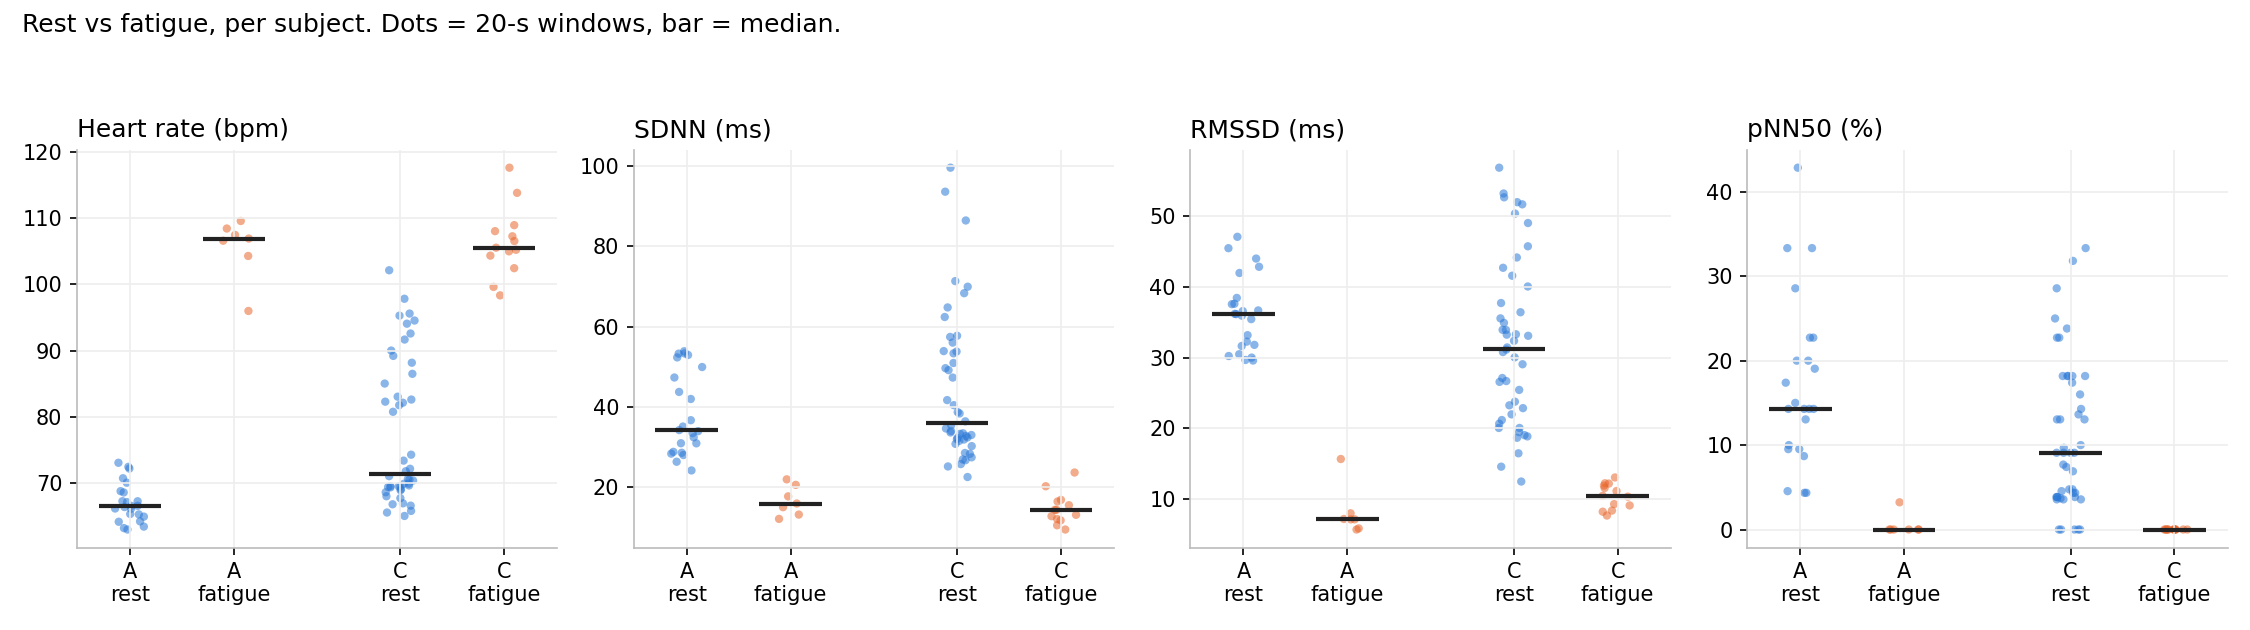
\includegraphics[width=0.95\linewidth]{11_rest_vs_fatigue.png}
\caption{Different resting levels, same shift: heart rate up, variability down, in both people (subject B is labelled C in this figure).}
\label{fig:shift}
\end{figure}

In absolute terms the two people look different. In \emph{percent} terms they look almost the same. That
became the heart of BreathBreak: every worker records a short \textbf{rested baseline} once, and every later
recording is described by how far it has moved from that baseline,
\[
x_{\text{HR}} = \ln\frac{\text{HR}_{\text{now}}}{\text{HR}_{\text{baseline}}},\quad
x_{\text{SDNN}} = \ln\frac{\text{SDNN}_{\text{now}}}{\text{SDNN}_{\text{baseline}}},\quad
x_{\text{RMSSD}} = \ln\frac{\text{RMSSD}_{\text{now}}}{\text{RMSSD}_{\text{baseline}}}.
\]

% =====================================================================
\section{Small model, big result}

With only a handful of recordings, a big model would simply memorise them. We chose the smallest model that
could express the idea: a \textbf{logistic regression on the three changes}, four parameters in total,
\[
P(\text{fatigue}) = \frac{1}{1+e^{-(b + w_{\text{HR}}\,z_{\text{HR}} + w_{\text{SDNN}}\,z_{\text{SDNN}} + w_{\text{RMSSD}}\,z_{\text{RMSSD}})}},
\]
where each $z$ is the standardised change. It learned exactly the physiology we expected: a positive weight
on heart rate ($+1.49$) and negative weights on SDNN ($-0.85$) and RMSSD ($-1.25$).

\paragraph{An honest test.} To avoid fooling ourselves, we used \emph{leave-one-out}: hide one recording,
train on all the others, score the hidden one against that person's rested baselines, and repeat until
every recording has been hidden once. Every score comes from a model that never saw that recording.

\begin{table}[h]
\centering
\caption{Leave-one-out on the 11 recordings made at healthy rest or during clear fatigue.}
\label{tab:loro}
\rowband\begin{tabular}{lll}
\toprule
Person & Recordings & P(fatigue) while hidden \\
\midrule
A, rest    & 2 & 0.06, 0.09 \\
A, fatigue & 5 & 0.62, 0.98, 0.99, 0.99, 1.00 \\
B, rest    & 3 & 0.02, 0.14, 0.25 \\
B, fatigue & 1 & 0.83 \\
\midrule
\multicolumn{3}{l}{\textbf{11/11 correct} at a 0.5 cutoff; no rested recording scored above 0.25.} \\
\bottomrule
\end{tabular}
\end{table}

Even better, the idea \emph{travelled}: trained only on B, the model classified all seven of A's recordings
correctly, and trained only on A it classified all four of B's.

\paragraph{Did big data help?} Our pitch promised a transfer-learning model: pre-train on public data
(WESAD stress \cite{wesad2018}, DROZY sleep deprivation \cite{drozy2016}), then fine-tune on ours. We built
it, and it did \emph{not} beat the small model (Table~\ref{tab:modelb}). WESAD's stress shifts in the right
direction but leans almost entirely on heart rate; DROZY's seated sleepiness barely moves HR or HRV at all, so
fine-tuning on it pulled the model the wrong way.

\begin{table}[h]
\centering
\caption{Model A (ours) vs.\ Model B (transfer learning), leave-one-out on our 11 recordings.}
\label{tab:modelb}
\rowband\begin{tabular}{lcc}
\toprule
Model & Correct & Brier (lower is better) \\
\midrule
\textbf{Model A: personal shift, logistic regression} & \textbf{11/11} & 0.025 \\
Model B: WESAD $\rightarrow$ DROZY $\rightarrow$ ours & 10/11 & 0.035 \\
Zero-shot: WESAD & 10/11 & 0.101 \\
Zero-shot: DROZY & 9/11 & 0.159 \\
\bottomrule
\end{tabular}
\end{table}

\lesson{a model is only as good as the question it asks. ``How far are you from \emph{your} rest?'' needed
four parameters; borrowing other people's stress and sleepiness did not help.}

% =====================================================================
\section{The plot twist: when ``normal'' is not normal}

Our dataset actually contained \textbf{14} recordings, not 11. Three of A's sessions were labelled
\emph{normal}, yet their heart rate was 105--109~bpm and their RMSSD as low as in A's fatigue sessions. We
had set them aside as ``not at rest''. When we looked closer, the explanation was simple and human:
\textbf{A was sick.} The fatigue sessions were noted as ``sick and tired'', and the ``normal'' ones were
recorded on the same evening, while A was still unwell.

Illness does to the heart much of what fatigue does. Fever alone raises resting heart rate by roughly
10~bpm per degree Celsius; the body's fight against infection pushes the nervous system towards its
sympathetic side, and heart-rate variability collapses. So A's ``feeling normal while sick'' already looked
like fatigue, and being tired on top of the illness barely changed anything.

\begin{twistbox}{\faExclamationTriangle\ \ Sick + tired $\approx$ sick alone}
\rowband\begin{tabular}{lccc}
\toprule
Subject A & Heart rate (bpm) & RMSSD (ms) & State \\
\midrule
Healthy rest & 65--69 & 33--39 & baseline \\
Sick, ``feeling normal'' (test file) & 105 & 8 & sick \\
Sick and tired (test file) & 100 & 12 & sick + fatigue \\
\bottomrule
\end{tabular}

\smallskip
Against A's \emph{healthy} rest, both sick recordings stand out (P = 0.95 and 0.88). Against each other, they
are \textbf{almost identical}: no heart-rate or HRV measure, and no baseline we tried, could separate them.
\end{twistbox}

We tested this as honestly as we could. Counting those three sick sessions as normal and re-running
leave-one-out on all 14 recordings, accuracy falls to \textbf{8/14 (57\%)}. We tried every one of A's
recordings as the baseline: a healthy baseline catches all six of A's fatigue recordings but flags the sick
``normals''; a sick baseline lets the sick ``normals'' pass but misses five or six of the six fatigues. On
every feature we compute (heart rate, HRV, R-peak height, T-wave ratio, R-to-T time) the two groups
overlap.

Subject B told the opposite story. B's fatigue came after \textbf{work and exertion}, measured against a
\textbf{healthy} baseline (69--88~bpm). There the shift is large and clean: B's fatigue recordings score
0.71--0.84, B's rested recordings at most 0.26.

\par\medskip\noindent\begin{minipage}{\linewidth}\centering
\includegraphics[page=6,width=0.82\linewidth]{breathbreak-slides.pdf}
\captionof{figure}{What kind of fatigue can we detect? Work fatigue against a healthy baseline: clearly.
Fatigue on top of illness: barely.}
\end{minipage}\par\medskip

\lesson{BreathBreak detects a \emph{shift away from a healthy, rested baseline}. Work and exertion fatigue
produce exactly that shift; illness produces it too. So baselines must be recorded while healthy, and an
alert during illness means ``you are far from your healthy self'', not necessarily ``you are tired from
work''. Our honest headline is therefore two numbers: \textbf{11/11} on recordings made at healthy rest or
clear fatigue, \textbf{57\%} when sessions recorded while sick are counted as normal.}

% =====================================================================
\section{Choosing which mistake to make}

Every alarm system trades two errors: raising an alarm when nothing is wrong (a \emph{false alarm}) and
staying silent when something is (a \emph{missed fatigue}). For BreathBreak we chose to make false alarms
the priority. A worker who is interrupted for nothing a few times will stop listening, and then even the
correct alerts are lost.

We built that choice into the system in two ways:
\begin{itemize}
  \item the alert threshold is \textbf{calibrated} to sit just above the highest score any held-out rested
  recording ever reached, so no rested recording in testing raises an alarm;
  \item only a \textbf{high} score counts: an alert needs $P(\text{fatigue})\ge 0.8$; what used to be
  ``moderate'' (0.5--0.8) is treated as normal.
\end{itemize}

\begin{table}[h]
\centering
\caption{The trade-off on the 11 reliably labelled recordings (board model, \texttt{board\_shift.py}).}
\rowband\begin{tabular}{lccc}
\toprule
Alert when & Accuracy & False alarms (of 5 rested) & Missed fatigue (of 6) \\
\midrule
$P\ge0.5$ & 11/11 (100\%) & 0 & 0 \\
$P\ge0.8$ (deployed) & 10/11 (91\%) & \textbf{0} & 1 (A, fatigue 5, the mildest: $P=0.62$) \\
\bottomrule
\end{tabular}
\end{table}

At the stricter setting the most fatigue-like rested recording (0.26) is far from the alarm line, and the
fatigue that slips through is the mildest one in the data. We accept that: BreathBreak is meant to catch
\emph{serious} fatigue without crying wolf. Zero false alarms on these five rested recordings (six, counting B's new test recording, which scores 0.24) is
encouraging but not proof; statistically it only bounds the false-alarm rate below roughly 40--50\%, and a convincing bound
needs dozens of rested recordings.

% =====================================================================
\section{Running at the edge}

The SK-AM62B runs Linux with Python and NumPy, but has no SciPy, no pandas, no Wi-Fi and no network cable.
So we made the whole pipeline fit what the board has:

\begin{itemize}
  \item We re-implemented zero-phase filtering and peak detection in pure NumPy. The board's pipeline matches
  the SciPy reference on the laptop to within $10^{-13}$.
  \item \texttt{board\_shift.py} is a single NumPy-only program that \textbf{trains} the model, runs the
  leave-one-out test, \textbf{enrolls} a new person's baseline and \textbf{checks} new recordings. Training on
  all our data takes about ten seconds; the model is a JSON file of a few kilobytes.
  \item With no network, we moved code and data over the 115{,}200-baud serial console: base64 chunks, each
  verified on the board with an MD5 checksum and re-sent if damaged, resumable after interruption.
\end{itemize}

Around it, a laptop dashboard in the colours of our slides lets a worker record a baseline, check a new
recording (NORMAL or FATIGUE, with the change in heart rate and HRV and a ``take a breath'' prompt), and
lets HR see fatigue alerts summarised by severity, never raw ECG.

\begin{center}

\begin{tikzpicture}[every node/.style={font=\sffamily\small}]
  \node[draw=bbnavy, fill=bbnavy, text=white, rounded corners=10pt, minimum width=3.4cm, minimum height=2.2cm, align=center]
    {\Large\bfseries FATIGUE\\[4pt]\colorbox{bbamber}{\color{bbnavy}\bfseries\ Take a breath\ }};
\end{tikzpicture}
\end{center}

% =====================================================================
\section{What we know, and what we don't}

\paragraph{What we can claim.}
\begin{itemize}
  \item Fatigue from work or exertion shows up as a large, consistent shift from a person's \emph{healthy}
  rest: heart rate up by roughly 40--60\%, RMSSD down by roughly 70--80\%.
  \item A four-parameter personal-shift model captures it: 11/11 in leave-one-out on reliably labelled
  recordings, with physiologically sensible weights, and it transfers between our two subjects.
  \item The whole thing trains and runs on the SK-AM62B with NumPy alone.
\end{itemize}

\paragraph{What we cannot claim yet.}
\begin{itemize}
  \item \textbf{Two people, 14 recordings.} Every number in this story rests on a very small study.
  \item \textbf{Illness and other causes.} Illness, exercise, stress or caffeine move heart rate and HRV the
  same way; with these three signals BreathBreak cannot tell them apart.
  \item \textbf{Mild fatigue.} A new, milder fatigue session in our technical report scored just below the
  line ($P\approx0.44$), and the stricter 0.8 alert level misses mild cases by design.
  \item \textbf{Short recordings, self-reported labels.} Several sessions are under a minute, below the
  5-minute HRV standard \cite{taskforce1996}, and labels were not backed by a sleepiness scale.
\end{itemize}

\paragraph{Next chapters.}
\begin{itemize}
  \item More people, each with 3--5 minute healthy-rest and fatigue sessions, labelled with the Karolinska
  Sleepiness Scale \cite{kss1990}, and a ``feeling sick?'' flag.
  \item More signals to separate illness from work fatigue: breathing rate derived from the ECG, PPG pulse
  timing, skin temperature, and how heart rate evolves over a shift.
  \item Live streaming from the AFE4950 into the board, alerting only on sustained fatigue (several
  fatigued windows in a row).
\end{itemize}

% =====================================================================
\section*{\color{bbnavy}Epilogue}

We started out wanting to detect fatigue. We ended up learning what our heartbeat actually tells us: not
``tired'' or ``not tired'', but \emph{how far you are from your healthy self}. For a worker at hour eleven,
after a long shift of honest work, that distance is large and clear, and BreathBreak can see it, on a
small board, without the cloud, without crying wolf.

\begin{center}
\begin{tcolorbox}[enhanced,width=0.8\linewidth,colback=bbnavy,colframe=bbnavy,arc=6pt,halign=center,
  fontupper=\sffamily\Large\itshape\color{white}]
{\color{bbamber}``}A small pause is better than a big accident.{\color{bbamber}''}
\end{tcolorbox}
\end{center}

% =====================================================================
\begin{thebibliography}{9}
\bibitem{williamson2000}
A.~M. Williamson and A.-M. Feyer, ``Moderate sleep deprivation produces impairments in cognitive and motor
performance equivalent to legally prescribed levels of alcohol intoxication,''
\emph{Occupational and Environmental Medicine}, 57(10):649--655, 2000.

\bibitem{taskforce1996}
Task Force of the ESC and NASPE, ``Heart rate variability: Standards of measurement, physiological
interpretation, and clinical use,'' \emph{Circulation}, 93(5):1043--1065, 1996.

\bibitem{shaffer2017}
F.~Shaffer and J.~P. Ginsberg, ``An overview of heart rate variability metrics and norms,''
\emph{Frontiers in Public Health}, 5:258, 2017.

\bibitem{pantompkins1985}
J.~Pan and W.~J. Tompkins, ``A real-time QRS detection algorithm,''
\emph{IEEE Trans.\ Biomedical Engineering}, BME-32(3):230--236, 1985.

\bibitem{wesad2018}
P.~Schmidt, A.~Reiss, R.~Duerichen, C.~Marberger, and K.~Van~Laerhoven, ``Introducing WESAD, a multimodal
dataset for wearable stress and affect detection,'' \emph{Proc.\ ICMI}, 2018.

\bibitem{drozy2016}
Q.~Massoz, T.~Langohr, C.~Fran\c{c}ois, and J.~G. Verly, ``The ULg multimodality drowsiness database
(called DROZY) and examples of use,'' \emph{Proc.\ IEEE WACV}, 2016.

\bibitem{kss1990}
T.~{\AA}kerstedt and M.~Gillberg, ``Subjective and objective sleepiness in the active individual,''
\emph{International Journal of Neuroscience}, 52(1--2):29--37, 1990.
\end{thebibliography}

\end{document}
